\documentclass[aspectratio=169]{beamer}

\setbeamersize{text margin left=5mm, text margin right=5mm}

\defbeamertemplate{headline}{my header}{%
\vskip1pt%
\makebox[0pt][l]{\,\insertshortauthor}%
\hspace*{\fill}\insertshorttitle/\insertshortsubtitle\hspace*{\fill}%
\llap{\insertpagenumber/\insertpresentationendpage\,}
}
\setbeamertemplate{headline}[my header]

\let\olditem\item
\renewcommand{\item}{\setlength{\itemsep}{\fill}\olditem}

\usepackage{caption}
\usepackage{soul}
\usepackage{tkz-euclide}
\usetikzlibrary{calc}
\usepackage[]{algorithm2e}
\usepackage{changepage}
\usepackage{amssymb}
\usepackage{xcolor}
\usepackage{mathtools}
\usepackage{tcolorbox}
\usepackage{tikz}
\usepackage{tikz-3dplot}
\usetikzlibrary{arrows.meta, decorations.pathreplacing, positioning, shapes.geometric}

%% Fonts
\usefonttheme{professionalfonts}
\usefonttheme{serif}

\DeclareCaptionLabelFormat{blank}{}
\captionsetup[figure]{labelformat=blank}

%% Math definitions
\def\mf{\ensuremath\mathbf}
\def\mb{\ensuremath\mathbb}
\def\lp{\ensuremath\left(}
\def\rp{\ensuremath\right)}
\def\lv{\ensuremath\left\lvert}
\def\rv{\ensuremath\right\rvert}
\def\lV{\ensuremath\left\lVert}
\def\rV{\ensuremath\right\rVert}
\def\lc{\ensuremath\left\{}
\def\rc{\ensuremath\right\}}
\def\ls{\ensuremath\left[}
\def\rs{\ensuremath\right]}
\def\bmx{\ensuremath\begin{bmatrix*}[r]}
\def\emx{\ensuremath\end{bmatrix*}}
\def\bmxc{\ensuremath\begin{bmatrix*}[c]}
\def\t{\lp t\rp}
\def\k{\ls k\rs}

\newcommand{\demoex}[2]{\onslide<#1->\begin{color}{black!60} #2 \end{color}}
\newcommand{\demoexc}[3]{\onslide<#1->\begin{color}{#2} #3 \end{color}}
\newcommand{\anim}[3]{\onslide<#1->{\begin{color}{#2!60} #3 \end{color}}}
\newcommand{\ct}[1]{\lp #1\rp}
\newcommand{\dt}[1]{\ls #1\rs}
\newcommand{\cols}[2]{\begin{columns}[#1] #2 \end{columns}}
\newcommand{\col}[2]{\begin{column}{#1} #2 \end{column}}

%% Mycolors
\definecolor{myred}{RGB}{192,0,0}
\definecolor{mygray}{RGB}{100,100,100}

%% Custom beamer color
\setbeamercolor{title}{fg=myred}
\setbeamercolor{subtitle}{fg=myred}
\setbeamerfont{title}{series=\bfseries}
% \setbeamercolor{frametitle}{bg=myred, fg=white}
\setbeamercolor{frametitle}{bg=mygray!10!, fg=myred}
\setbeamerfont{frametitle}{series=\bfseries}
\setbeamercolor{item}{fg=mygray}
\setbeamercolor{title in head/foot}{fg=myred}

% Move header to footer
\setbeamertemplate{headline}{}
\setbeamertemplate{footline}{
  \begin{beamercolorbox}[wd=\paperwidth,ht=2.25ex,dp=1ex,center]{footline}
    \inserttitle\hfill\insertauthor\hfill\insertdate\hfill\insertframenumber{}
  \end{beamercolorbox}
}

\title{Applied Linear Algebra in Data Analysis}

% A subtitle is optional and this may be deleted
\subtitle{Case Study 01}

\author{Sivakumar Balasubramanian}
% - Give the names in the same order as the appear in the paper.
% - Use the \inst{?} command only if the authors have different
%   affiliation.

\institute[Christian Medical College] % (optional, but mostly needed)
{
  \inst{}%
  Department of Bioengineering\\
  Christian Medical College, Bagayam\\
  Vellore 632002
}
% - Use the \inst command only if there are several affiliations.
% - Keep it simple, no one is interested in your street address.

\date{}
% - Either use conference name or its abbreviation.
% - Not really informative to the audience, more for people (including
%   yourself) who are reading the slides online

\subject{Lecture notes on ALADA}
% This is only inserted into the PDF information catalog. Can be left
% out. 

% If you have a file called "university-logo-filename.xxx", where xxx
% is a graphic format that can be processed by latex or pdflatex,
% resp., then you can add a logo as follows:

% \pgfdeclareimage[height=0.5cm]{university-logo}{university-logo-filename}
% \logo{\pgfuseimage{university-logo}}

% Delete this, if you do not want the table of contents to pop up at
% the beginning of each subsection:
\AtBeginSubsection[]
{
  \begin{frame}<beamer>{Outline}
    \tableofcontents[currentsection,currentsubsection]
  \end{frame}
}

% Let's get started
\begin{document}

\begin{frame}
  \titlepage
\end{frame}


\begin{frame}[t]{What is this case study about?}
\begin{itemize}
\item We will apply some of the concepts we have learned from the Vectors space, Matrcies, and Solutions to Linear Equations modules.
\item We will be working with text data for this case study, in particular doctors' notes/reports from different specialities.
\item We want to used these reports for two purposes:
\begin{enumerate}
  \item Cluster the set of reports into similar groups -- to possibly identify which specialities these reports might be from.
  \item To use to reports to learn the relationship between different medical terms/concepts.
\end{enumerate}
\item We will make use of a dataset from kaggle for this case study: \href{https://www.kaggle.com/datasets/gauravmodi/doctors-notes/data}{https://www.kaggle.com/datasets/gauravmodi/doctors-notes/data}
\end{itemize}
\end{frame}


\begin{frame}[t]{Clustering of doctors' notes}
  \textbf{Clustering}: Grouping similar items together.

  \begin{itemize}
    \item There are various clustering algorithms: k-means, hierarchical clustering, Gaussian mixture models, etc.
    \item \textbf{k-means} is the simplest and most popular clustering algorithm.
  \end{itemize}

  \begin{figure}
    \centering
    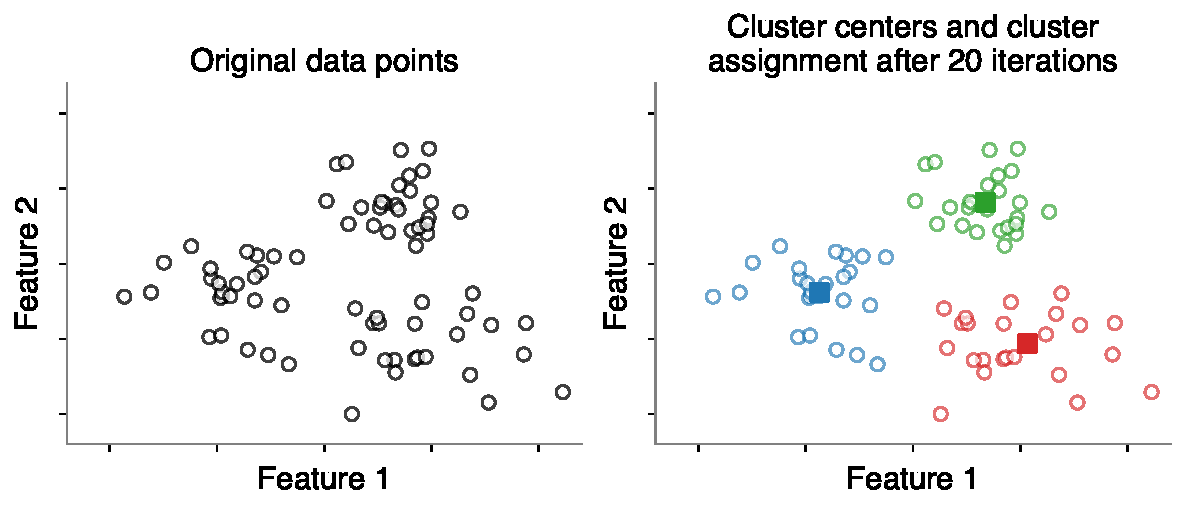
\includegraphics[width=0.7\textwidth]{kmeans-final.pdf}
  \end{figure}
\end{frame}


\begin{frame}[t]{k-means clustering}
  \begin{itemize}
    \item The k-means algorithm is an iterative algorithm that divides a group of $N$ samples ($n$-vectors) into $k$ clusters.

    \item Clustering is done by minimizing the following cost,
    \[ J_{clust} = \frac{1}{N}\sum_{j=1}^k \sum_{i \in C_j} \lV \mf{x}_i - \mf{m}_j \rV_2^2 \]
  
    \item Minimizing this cost for a given dataset is computational intensive, because the optimal choice for the means $\mf{m}_j$ and the cluster assignments $C_j$ depend on each other.
    
    \item k-means takes a simpler approach: minimizing $J_{clust}$ when either the means or the cluster assignments are fixed is easy. 
  \end{itemize}
\end{frame}


\begin{frame}[t]{k-means clustering}
  \begin{itemize}
    \item k-means solves the clustering problem by minimizing $J_clust$ by alternatively fixing the means and the cluster assignments, while updating the other.
    \item k-means has two steps: we first randomly choose some cluster means.
    \begin{itemize}
      \item \textbf{Cluster assignment update}: For a fixed set of cluster means, find cluster assignments that minimize $J_{clust}$.
      \item \textbf{Cluster means update}: For a fixed cluster assignment, find the means $\mf{m}_i$ that miimize $J_{clust}$.
    \end{itemize}
    \item Applying these two steps one after the other will lead to the algorithm converging towards a set of cluster means and assignments, because $J_{clust}$ is guarnteed to reduce with each step.
  \end{itemize}
\end{frame}


\begin{frame}[t]{k-means clustering}
  \begin{figure}
    \centering
    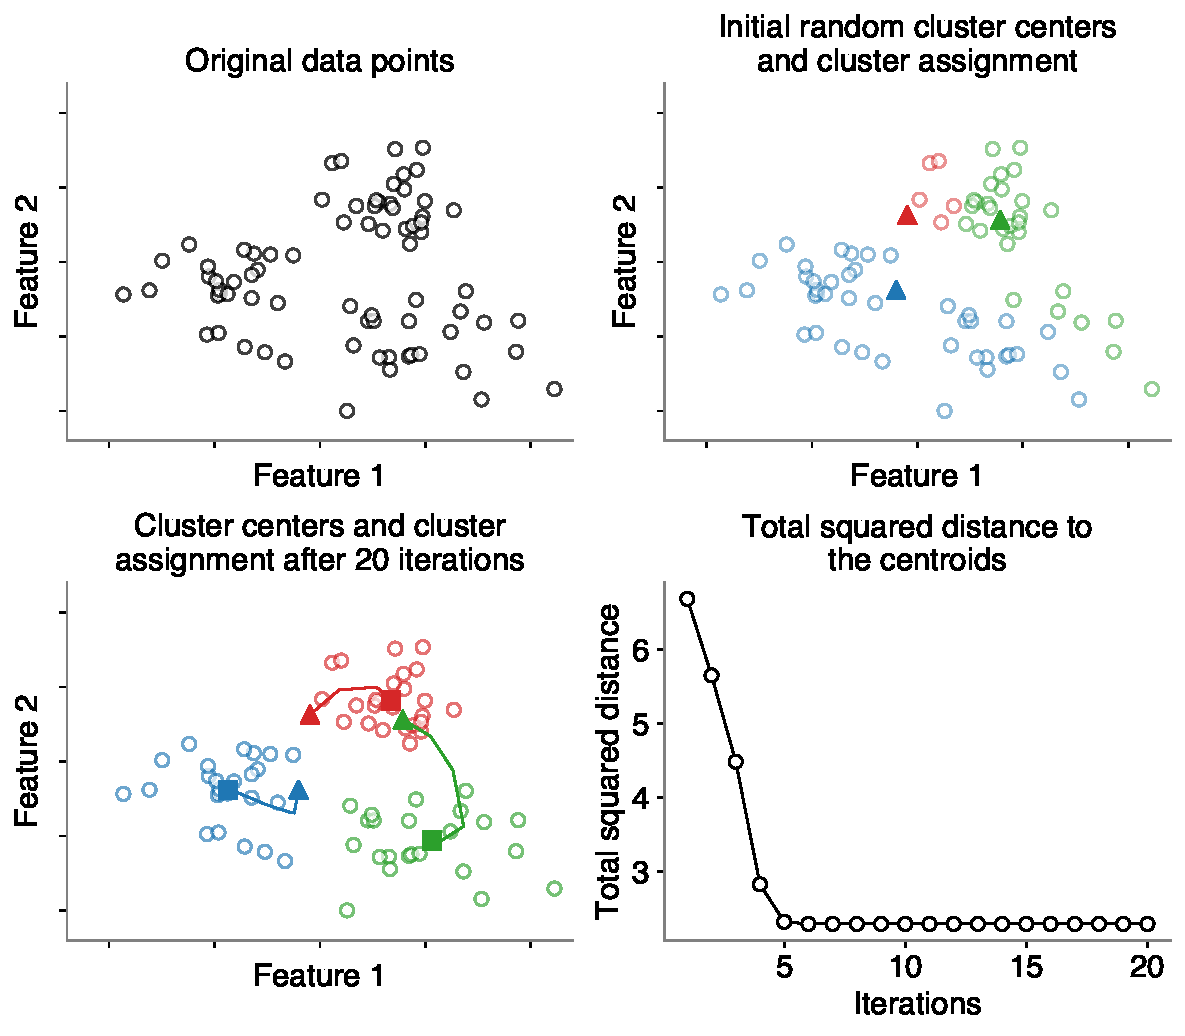
\includegraphics[width=0.525\textwidth]{kmeans-algo.pdf}
  \end{figure}
\end{frame}


\begin{frame}[t]{Clustering of doctors' notes}
  The details of this case study is in the \texttt{case\_study\_01.ipynb} file, which can be found in the \texttt{case\_studies} folder.

  The rest of the details are in the .ipynb file.
\end{frame}


\begin{frame}[t]{Case Study 01b: Co-occurence graph of medical terms}
  \begin{itemize}
    \item Co-coccurence network or graph is a graph representing the relationship between different terms/concepts/keywords.
    \item The nodes of the graph are the terms and the edges represent a measure of how often two terms occur together in a text, sentence, etc.
    \item A co-occurence graph can be learned from a set of text blobs or documents containing the terms/keywords of interest.
    \item The details of this case study is in the \texttt{case\_study\_01b.ipynb} file, which can be found in the \texttt{case\_studies} folder.

    
    The rest of the details are in the .ipynb file.
  \end{itemize}
\end{frame}

\end{document}